% Options for packages loaded elsewhere
\PassOptionsToPackage{unicode}{hyperref}
\PassOptionsToPackage{hyphens}{url}
\documentclass[
  ignorenonframetext,
]{beamer}
\newif\ifbibliography
\usepackage{pgfpages}
\setbeamertemplate{caption}[numbered]
\setbeamertemplate{caption label separator}{: }
\setbeamercolor{caption name}{fg=normal text.fg}
\beamertemplatenavigationsymbolsempty
% remove section numbering
\setbeamertemplate{part page}{
  \centering
  \begin{beamercolorbox}[sep=16pt,center]{part title}
    \usebeamerfont{part title}\insertpart\par
  \end{beamercolorbox}
}
\setbeamertemplate{section page}{
  \centering
  \begin{beamercolorbox}[sep=12pt,center]{section title}
    \usebeamerfont{section title}\insertsection\par
  \end{beamercolorbox}
}
\setbeamertemplate{subsection page}{
  \centering
  \begin{beamercolorbox}[sep=8pt,center]{subsection title}
    \usebeamerfont{subsection title}\insertsubsection\par
  \end{beamercolorbox}
}
% Prevent slide breaks in the middle of a paragraph
\widowpenalties 1 10000
\raggedbottom
\AtBeginPart{
  \frame{\partpage}
}
\AtBeginSection{
  \ifbibliography
  \else
    \frame{\sectionpage}
  \fi
}
\AtBeginSubsection{
  \frame{\subsectionpage}
}
\usepackage{iftex}
\ifPDFTeX
  \usepackage[T1]{fontenc}
  \usepackage[utf8]{inputenc}
  \usepackage{textcomp} % provide euro and other symbols
\else % if luatex or xetex
  \usepackage{unicode-math} % this also loads fontspec
  \defaultfontfeatures{Scale=MatchLowercase}
  \defaultfontfeatures[\rmfamily]{Ligatures=TeX,Scale=1}
\fi
\usepackage{lmodern}
\ifPDFTeX\else
  % xetex/luatex font selection
\fi
% Use upquote if available, for straight quotes in verbatim environments
\IfFileExists{upquote.sty}{\usepackage{upquote}}{}
\IfFileExists{microtype.sty}{% use microtype if available
  \usepackage[]{microtype}
  \UseMicrotypeSet[protrusion]{basicmath} % disable protrusion for tt fonts
}{}
\makeatletter
\@ifundefined{KOMAClassName}{% if non-KOMA class
  \IfFileExists{parskip.sty}{%
    \usepackage{parskip}
  }{% else
    \setlength{\parindent}{0pt}
    \setlength{\parskip}{6pt plus 2pt minus 1pt}}
}{% if KOMA class
  \KOMAoptions{parskip=half}}
\makeatother
\usepackage{graphicx}
\makeatletter
\newsavebox\pandoc@box
\newcommand*\pandocbounded[1]{% scales image to fit in text height/width
  \sbox\pandoc@box{#1}%
  \Gscale@div\@tempa{\textheight}{\dimexpr\ht\pandoc@box+\dp\pandoc@box\relax}%
  \Gscale@div\@tempb{\linewidth}{\wd\pandoc@box}%
  \ifdim\@tempb\p@<\@tempa\p@\let\@tempa\@tempb\fi% select the smaller of both
  \ifdim\@tempa\p@<\p@\scalebox{\@tempa}{\usebox\pandoc@box}%
  \else\usebox{\pandoc@box}%
  \fi%
}
% Set default figure placement to htbp
\def\fps@figure{htbp}
\makeatother
\setlength{\emergencystretch}{3em} % prevent overfull lines
\providecommand{\tightlist}{%
  \setlength{\itemsep}{0pt}\setlength{\parskip}{0pt}}
% Slide layout defaults for warning-clean scientific decks.
\usepackage{etoolbox}
\IfFileExists{xurl.sty}{\usepackage{xurl}}{}
\IfFileExists{seqsplit.sty}{\usepackage{seqsplit}}{\newcommand{\seqsplit}[1]{#1}}
\protected\def\breakseq#1{\seqsplit{#1}}
\protected\def\breaktt#1{\begingroup\ttfamily\seqsplit{#1}\endgroup}
\setlength{\emergencystretch}{6em}
\tolerance=5000
\hbadness=10000
\hfuzz=1pt
\setlength{\tabcolsep}{2pt}
\AtBeginEnvironment{longtable}{\tiny\renewcommand{\arraystretch}{0.86}\setlength{\tabcolsep}{1pt}}
\AtBeginEnvironment{tabular}{\tiny\renewcommand{\arraystretch}{0.86}\setlength{\tabcolsep}{1pt}}

% Natbib and cross-reference fallbacks — slides don't load natbib
% or cleveref, but combined-PDF manuscript prose may emit these
% commands. The fallback renders citations as a bracketed key list
% and cross-references as detokenized labels so slides don't fail on
% undefined control sequences or raw underscores. \providecommand is
% a no-op if packages load later.
\providecommand{\citep}[1]{[#1]}
\providecommand{\citet}[1]{#1}
\providecommand{\citealp}[1]{#1}
\providecommand{\citeauthor}[1]{#1}
\providecommand{\citeyear}[1]{#1}
\providecommand{\cref}[1]{\texttt{\detokenize{#1}}}
\providecommand{\Cref}[1]{\texttt{\detokenize{#1}}}

\newtheorem{proposition}{Proposition}
\newtheorem{hypothesis}{Hypothesis}
\usepackage{bookmark}
\IfFileExists{xurl.sty}{\usepackage{xurl}}{} % add URL line breaks if available
\urlstyle{same}
% fallback for those not using the hyperref driver hyperxmp:
\makeatletter
\@ifundefined{xmpquote}{\newcommand{\xmpquote}[1]{#1}}{}
\makeatother
\hypersetup{
  hidelinks,
  pdfcreator={LaTeX via pandoc}}

\author{\texorpdfstring{}{}}
\date{}

\begin{document}

\section{Research Agenda: From Feasibility to
Evidence}\label{sec:agenda}

\begin{frame}[fragile,allowframebreaks]{Research Agenda: From
Feasibility to Evidence}
The framework identifies a large research program.
\breakseq{[@fig:research\_agenda]} condenses it into priorities that can be run
as staged studies rather than as a single overbroad claim. The first
priority is modality comparison: co-present paper PPPiP, synchronous
remote DigiPPPiP, semisynchronous drawing, and asynchronous
persistent-canvas practice should be compared on relational,
phenomenological, behavioral, accessibility, and narrative outcomes. The
comparison should include matched controls such as ordinary shared
drawing, video chat, shared games, and solo art-making so DigiPPPiP is
not credited for effects that any pleasant shared activity would
produce.

\begin{figure}
\centering
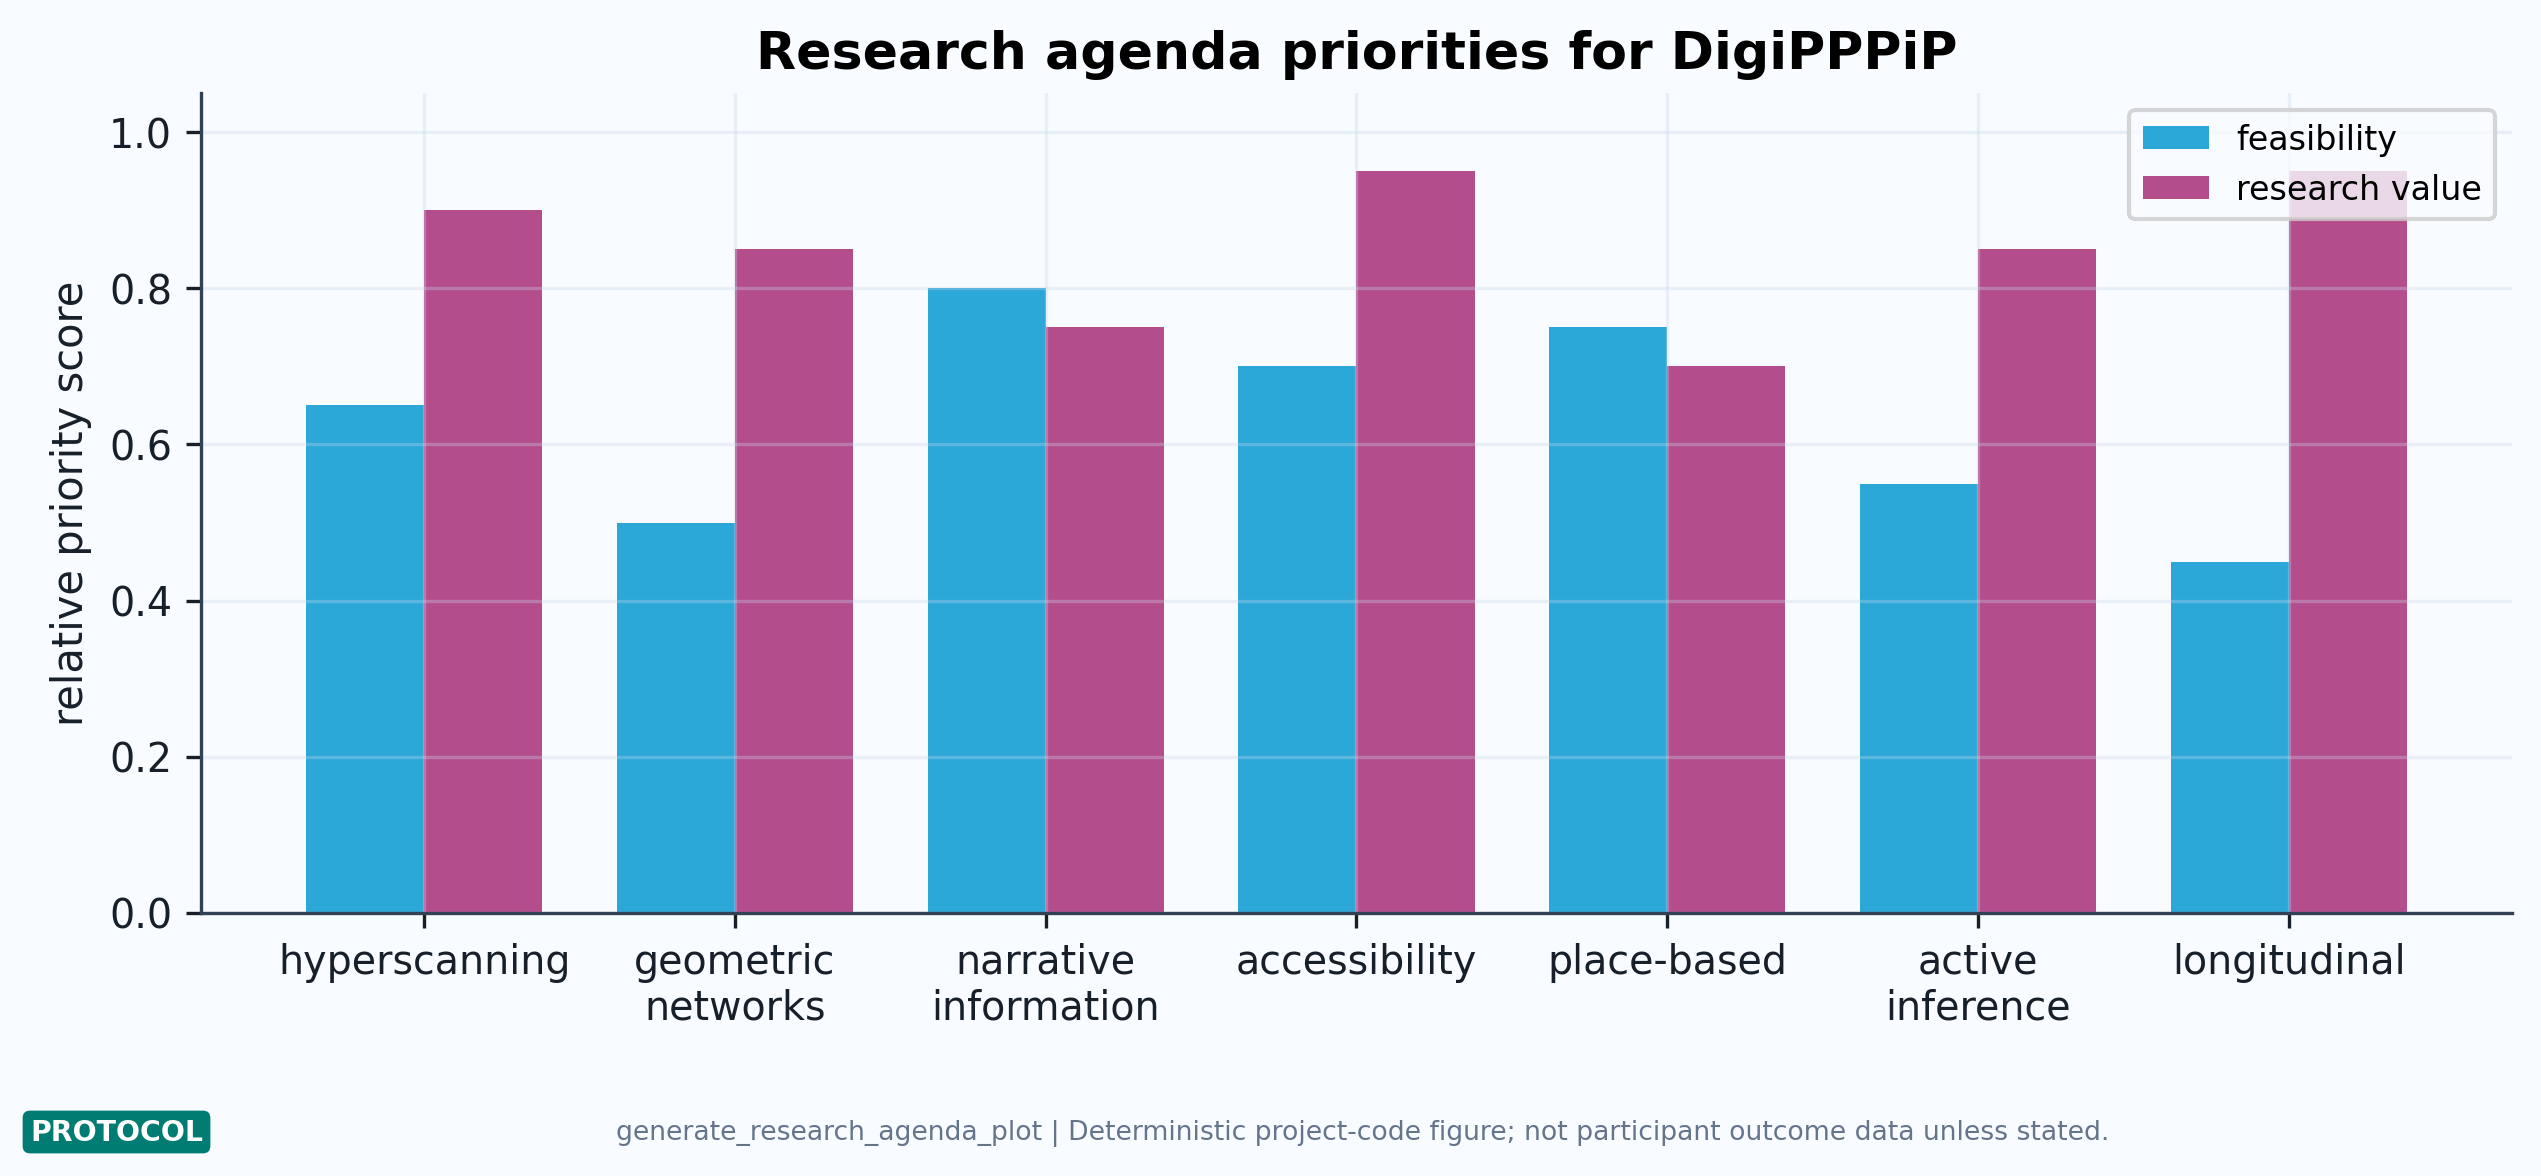
\includegraphics[width=0.9\linewidth,height=0.46\textheight,keepaspectratio,alt={Conceptual research-priority map for DigiPPPiP. The figure is generated by generate\_research\_agenda\_plot(); read paired bars as relative feasibility and research value assigned by the framework design for each agenda item. It supports staged prioritization rather than external funding or outcome claims. The values are conceptual planning scores, and future versions should replace them with feasibility data, stakeholder priorities, and study results.}]{../figures/research_agenda.png}
\caption{Conceptual research-priority map for DigiPPPiP. The figure is
generated by \protect\breaktt{generate\_research\_agenda\_plot()}; read
paired bars as relative feasibility and research value assigned by the
framework design for each agenda item. It supports staged prioritization
rather than external funding or outcome claims. The values are
conceptual planning scores, and future versions should replace them with
feasibility data, stakeholder priorities, and study
results.}\label{fig:research_agenda}
\end{figure}

The staged path should begin with feasibility and meaning before
physiology, following the validation ladder in
\breakseq{[@fig:validation\_ladder]}. Early studies should ask whether partners
understand the task, preserve consent, use the canvas intentionally, and
describe the artifacts as relationally meaningful. Only after those
conditions hold should instrumentation-heavy studies test neural,
narrative, or active-inference hypotheses. This ordering follows from
the design kernel: no signal-processing result can rescue a practice
that participants do not experience as shared agency.

The systems-governance agenda should be tested alongside the outcome
agenda. A pilot should record whether partners use save, replay,
redaction, deletion, and export controls; whether place prompts are
accepted, declined, or coarsened; whether accessibility accommodations
change during the session; and whether optional AI suggestions are
ignored, rejected, revised, or treated as partner-like. These are not
secondary usability details. They are the feedback signals that decide
whether the framework's branches remain reversible and ethically
bounded.

Hyperscanning studies should test whether the phase structure in
\breakseq{[@fig:ibs\_phases]} appears in real dyads. Geometric-hyperscanning
studies should evaluate whether the appendix's curvature proxy tracks
rupture, repair, or co-regulation events after the artifact and
alignment limits are addressed \breakseq{[@sec:formalisms\_appendix]}.
Narrative-information studies should test whether the appendix's entropy
and surprisal primitives predict partners' reports of novelty,
coherence, or shared meaning \breakseq{[@schulz2024narrativeinfo]}.

Accessibility research should be participatory from the start. Disabled
partners should help define input modes, feedback channels, consent
controls, and successful participation. Place-based studies should test
whether place-responsive prompts increase place attachment or relational
memory compared with non-place prompts \breakseq{[@lewicka2011place]}.

AI-assisted studies need a separate preregistered logic.
Mixed-initiative interfaces can join automated suggestions with direct
manipulation, but that does not make automation harmless or
relationship-preserving \breakseq{[@horvitz1999mixedinitiative;
@deterding2017mixedinitiative]}. AI-mediated communication scholarship
is especially relevant because it treats AI as modifying, augmenting, or
generating interpersonal messages on behalf of a communicator, with
consequences for agency, trust, relationship interpretation, and ethics
\breakseq{[@hancock2020aimediatedcommunication]}. Companion-AI scholarship adds
a distinct replacement and social-deskilling concern, so AI-supported
DigiPPPiP should be measured against whether it strengthens human-human
attention rather than satisfying a user through the system itself
\breakseq{[@malfacini2025companionai]}. Human-AI interaction guidelines imply
concrete requirements for DigiPPPiP: disclose what the model can and
cannot do, let partners accept, reject, revise, or undo suggestions,
support efficient dismissal, and recover gracefully from wrong or
intrusive prompts \breakseq{[@amershi2019humanai]}. If the AI branch becomes a
clinical or health-intervention trial, the Consolidated Standards of
Reporting Trials for AI (CONSORT-AI) and the Standard Protocol Items for
AI trials (SPIRIT-AI) extensions require AI-specific descriptions of the
intervention, input and output data, human-AI interaction, errors, and
use setting \breakseq{[@liu2020consortai; @cruzrivera2020spiritai]}. Even
outside a trial, the optional branch should maintain a risk log using
the National Institute of Standards and Technology Artificial
Intelligence Risk Management Framework (NIST AI RMF) concepts and check
whether any deployed system would fall within European Union (EU) AI Act
obligations \breakseq{[@nist2023airmf; @europeanunion2024aiact]}. Empirical
medical-AI ethics reviews add a further caution: high-level ethical
principles often fail to match stakeholder experience unless patients,
clinicians, developers, and ethics expertise are involved in the design
and evaluation process \breakseq{[@tang2023medicalaiethics]}. The outcome
question is not whether AI makes drawings more polished. It is whether
AI helps partners notice each other, preserve co-authorship, and discuss
uncertainty without outsourcing imagination, authorship, or emotional
interpretation.

Longitudinal studies should compare DigiPPPiP with matched shared
activities such as video calls, shared games, text messaging,
relatedness-technology prototypes, or shared media consumption
\breakseq{[@wenhart2025relatedness]}. The comparison set should include at
least one lightweight routine and one richer sensory or gestural system,
because affective textile systems for long-distance partners show how
non-visual gesture channels can address needs that a drawing canvas may
not meet \breakseq{[@jiang2025ipillowpal]}. No single method can validate the
framework; the research agenda has to triangulate logs, interviews,
accessibility audits, relational outcomes, privacy acceptability, and
optional physiology.
\end{frame}

\end{document}
